% -*- coding:utf-8 -*-
\documentclass{standalone}
\usepackage[UTF8]{ctex}
\usepackage{tikz}
\usepackage{amsmath}
\usetikzlibrary{matrix,calc,shapes,backgrounds,patterns,positioning,decorations.pathreplacing}
\begin{document}
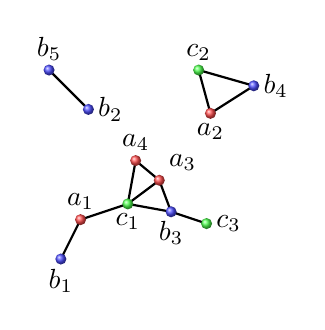
\begin{tikzpicture}
%draw the grid
% \foreach \x in {0,..., 6}
% 	\draw[style=dashed,-] (0.5*\x,0) -- (0.5*\x, 3);
% \foreach \x in {0,..., 6}	
% 	\draw[style=dashed,-] (0, 0.5*\x) -- (3, 0.5*\x);
% %draw the coordinate
% \foreach \x in {1,...,6}
% 	\node[below] at (0.5*\x-0.25,0){\x};
% \foreach \x in {1,...,6}
% 	\node[left] at (0, 0.5*\x -0.25){\x};
%first 
\draw[thick, -] (0.7/2, 5.3/2) -- (1.7/2, 4.3/2);
\shade[shading=ball, ball color=blue!70] (0.7/2, 5.3/2) circle (2pt) node[above]{$b_5$};
\shade[shading=ball, ball color=blue!70] (1.7/2, 4.3/2) circle (2pt) node[right]{$b_2$};

% %second
\draw[thick, -] (4.5/2, 5.3/2) --  (4.8/2, 4.2/2) -- (5.9/2,  4.9/2) -- cycle;
\shade[shading=ball, ball color=green!70] (4.5/2, 5.3/2) circle (2pt) node[above]{$c_2$};
\shade[shading=ball, ball color=red!70] (4.8/2, 4.2/2) circle (2pt) node[below]{$a_2$};
\shade[shading=ball, ball color=blue!70] (5.9/2,  4.9/2) circle(2pt) node[right]{$b_4$};

% %draw last
\draw[thick, -] (1/2, 0.5/2) -- (1.5/2, 1.5/2) -- (2.7/2, 1.9/2) -- (2.9/2, 3.0/2) -- (3.5/2, 2.5/2) -- (3.8/2, 1.7/2) -- (4.7/2, 1.4/2);
\draw[thick, -] (3.8/2, 1.7/2)  -- (2.7/2, 1.9/2)  -- (3.5/2, 2.5/2) ;
\shade[shading=ball, ball color=blue!70] (1/2, 0.5/2) circle (2pt) node[below]{$b_1$};
\shade[shading=ball, ball color=red!70] (1.5/2, 1.5/2) circle (2pt) node[above]{$a_1$};
\shade[shading=ball, ball color=green!70] (2.7/2, 1.9/2) circle (2pt) node[below]{$c_1$};
\shade[shading=ball, ball color=red!70] (2.9/2, 3.0/2) circle (2pt) node[above]{$a_4$};
\shade[shading=ball, ball color=red!70] (3.5/2, 2.5/2) circle (2pt) node[above right]{$a_3$};
\shade[shading=ball, ball color=blue!70] (3.8/2, 1.7/2) circle(2pt) node[below]{$b_3$};
\shade[shading=ball, ball color =green!70] (4.7/2, 1.4/2) circle(2pt) node[right]{$c_3$};
%draw the row instances
% \draw[very thick, ->] (3.1, 1.5) -- (3.4, 1.5);
% \draw[thick, -] (3.5, 3) -- (4.5, 3);
% \node at (3.75, 2.875) {\tiny A1}; \node at (4.25, 2.875) {\tiny B1};
% \node at (3.75, 2.625) {\tiny A1}; \node at (4.25, 2.625) {\tiny C1};
% \node at (3.75, 2.375) {\tiny C1}; \node at (4.25, 2.375) {\tiny B3};
% \node at (3.75, 2.125) {\tiny C1}; \node at (4.25, 2.125) {\tiny A4};
% \node at (3.75, 1.875) {\tiny A4}; \node at (4.25, 1.875) {\tiny A3};
% \node at (3.75, 1.625) {\tiny A3}; \node at (4.25, 1.625) {\tiny C1};
% \node at (3.75, 1.375) {\tiny B3}; \node at (4.25, 1.375) {\tiny C3};
% \node at (3.75, 1.125) {\tiny B3}; \node at (4.25, 1.125) {\tiny B3};
% \node at (3.75, .875) {\tiny A2}; \node at (4.25, 0.875) {\tiny B4};
% \node at (3.75, 0.625) {\tiny A2}; \node at (4.25, 0.625) {\tiny C2};
% \node at (3.75, 0.375) {\tiny C2}; \node at (4.25, 0.375) {\tiny B4};
% \node at (3.75, 0.125) {\tiny B5}; \node at (4.25, 0.125) {\tiny B2};
% \node[below] at (4, 0) {\tiny 二阶行实例};
% %draw the table instance
% \draw[very thick, ->] (4.6, 1.5) -- (4.9, 1.5);
% \draw[thick, -] (5, 3.25) -- (6,3.25);
% \node at (5.25, 3.125){\tiny A}; \node at (5.75, 3.125){\tiny B};
% \draw[style=dashed,  - ] (5, 3)--(6, 3);
% \node at (5.25, 2.875) {\tiny A1}; \node at (5.75, 2.875) {\tiny B1};
% \node at (5.25, 2.625) {\tiny A3}; \node at (5.75, 2.625) {\tiny B3};
% \node at (5.25, 2.375) {\tiny A2}; \node at (5.75, 2.375) {\tiny B4};
% \draw[thick, -] (5, 2.25) -- (6,2.25);
% \node at (5.25, 2.125) {\tiny A}; \node at (5.75, 2.125) {\tiny C};
% \draw[style=dashed,  - ] (5, 2)--(6, 2);
% \node at (5.25, 1.875) {\tiny A4}; \node at (5.75, 1.875) {\tiny C1};
% \node at (5.25, 1.625) {\tiny A1}; \node at (5.75, 1.625) {\tiny C1};
% \node at (5.25, 1.375) {\tiny A3}; \node at (5.75, 1.375) {\tiny C1};
% \node at (5.25, 1.125) {\tiny A2}; \node at (5.75, 1.125) {\tiny C2};
% \draw[thick, -] (5, 1) -- (6,1);
% \node at (5.25, .875) {\tiny B}; \node at (5.75, 0.875) {\tiny C};
% \draw[style=dashed,  - ] (5, 0.75)--(6, 0.75);
% \node at (5.25, 0.625) {\tiny B3}; \node at (5.75, 0.625) {\tiny C1};
% \node at (5.25, 0.375) {\tiny B3}; \node at (5.75, 0.375) {\tiny C3};
% \node at (5.25, 0.125) {\tiny B4}; \node at (5.75, 0.125) {\tiny C2};
%\node[below] at (5.5,0) {\tiny 二阶表实例};
\end{tikzpicture}
\end{document}